\chapter{Zadanie 3.}
Odpowied� skokowa zosta�a zebrana poprzez zmian� sterowania z $ u = U_{pp} = 2 $ na $ u = 2.8 $ i zebranie odpowiedzi obiektu. Poniewa� odpowied� skokowa, u�ywana w algorytmie DMC jest odpowiedzi� na skok jednostkowy z sygna�u sterowania r�wnego zero, nale�a�o j� znormalizowa� zgodnie z poni�szym wzorem:
$$ s = \frac{s_{0} - Y_{pp}}{\Delta u} $$
gdzie:
\begin{itemize}
\item $ s $ - znormalizowana odpowied� skokowa
\item $ s_{0} $ - zebrana odpowied� skokowa
\item $ Y_{pp} $ - wyj�cie uk�adu w punkcie pracy
\item $ \Delta u $ - warto�� skoku sterowania
\end{itemize}

Otrzymana odpowied� skokowa po normalizacji wygl�da nast�puj�co:
\begin{figure}[b]
\centering
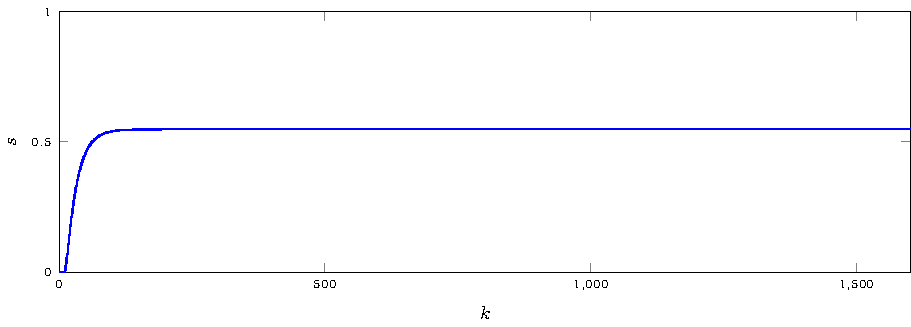
\includegraphics[scale=1]{rysunki/zapisz_pdf/proj1/odpowiedz_skokowa.pdf}
\caption {Odpowied� skokowa}
\end{figure}